\chapter{Localization}

As mentioned in Chapter \ref{intro_localization}, localization is the process of determining the current robot position using the measurements up to the 
current instant.\\
In the first section we will describe the Differential Drive technique, which uses the encoder measurements; in the second section we will describe the Inertial Navigation technique, which uses the IMU measurements.

\section{Differential Drive}

Differential Drive\supercite{diff_drive} is a localization technique consisting in calculating the odometry of the robot from the instant rotation of each wheel. In the following we will assume 2 drive wheels mounted on the same axis, and we will take the center of the robot on the mid-point of the wheel axis.\\
We will call, \textit{b} the length of the basis of the robot (i.e. the length of the wheel axis) and \textit{C} the center of the robot.\\

We use the two rotary encoders to have measurements about the wheels' rotations. We sample the values of the encoders at 100 Hz. Knowing the radius of each wheel, we can then compute the distance traveled by each wheel every 10ms starting from the corresponding measured rotation.\\
In the following we will call \textit{l, r} the distance traveled by the left and by the right wheel respectively.\\

\subsection{Movement in the Local Reference Frame}

We can model each instant movement as a rotation of an angle $\alpha$ around a point \textit{O} lying on the wheel axis, at a distance \textit{R} from the center of the robot (note that \textit{R} will be the radius of the robots' rotation).\\
\begin{figure}[!ht]
	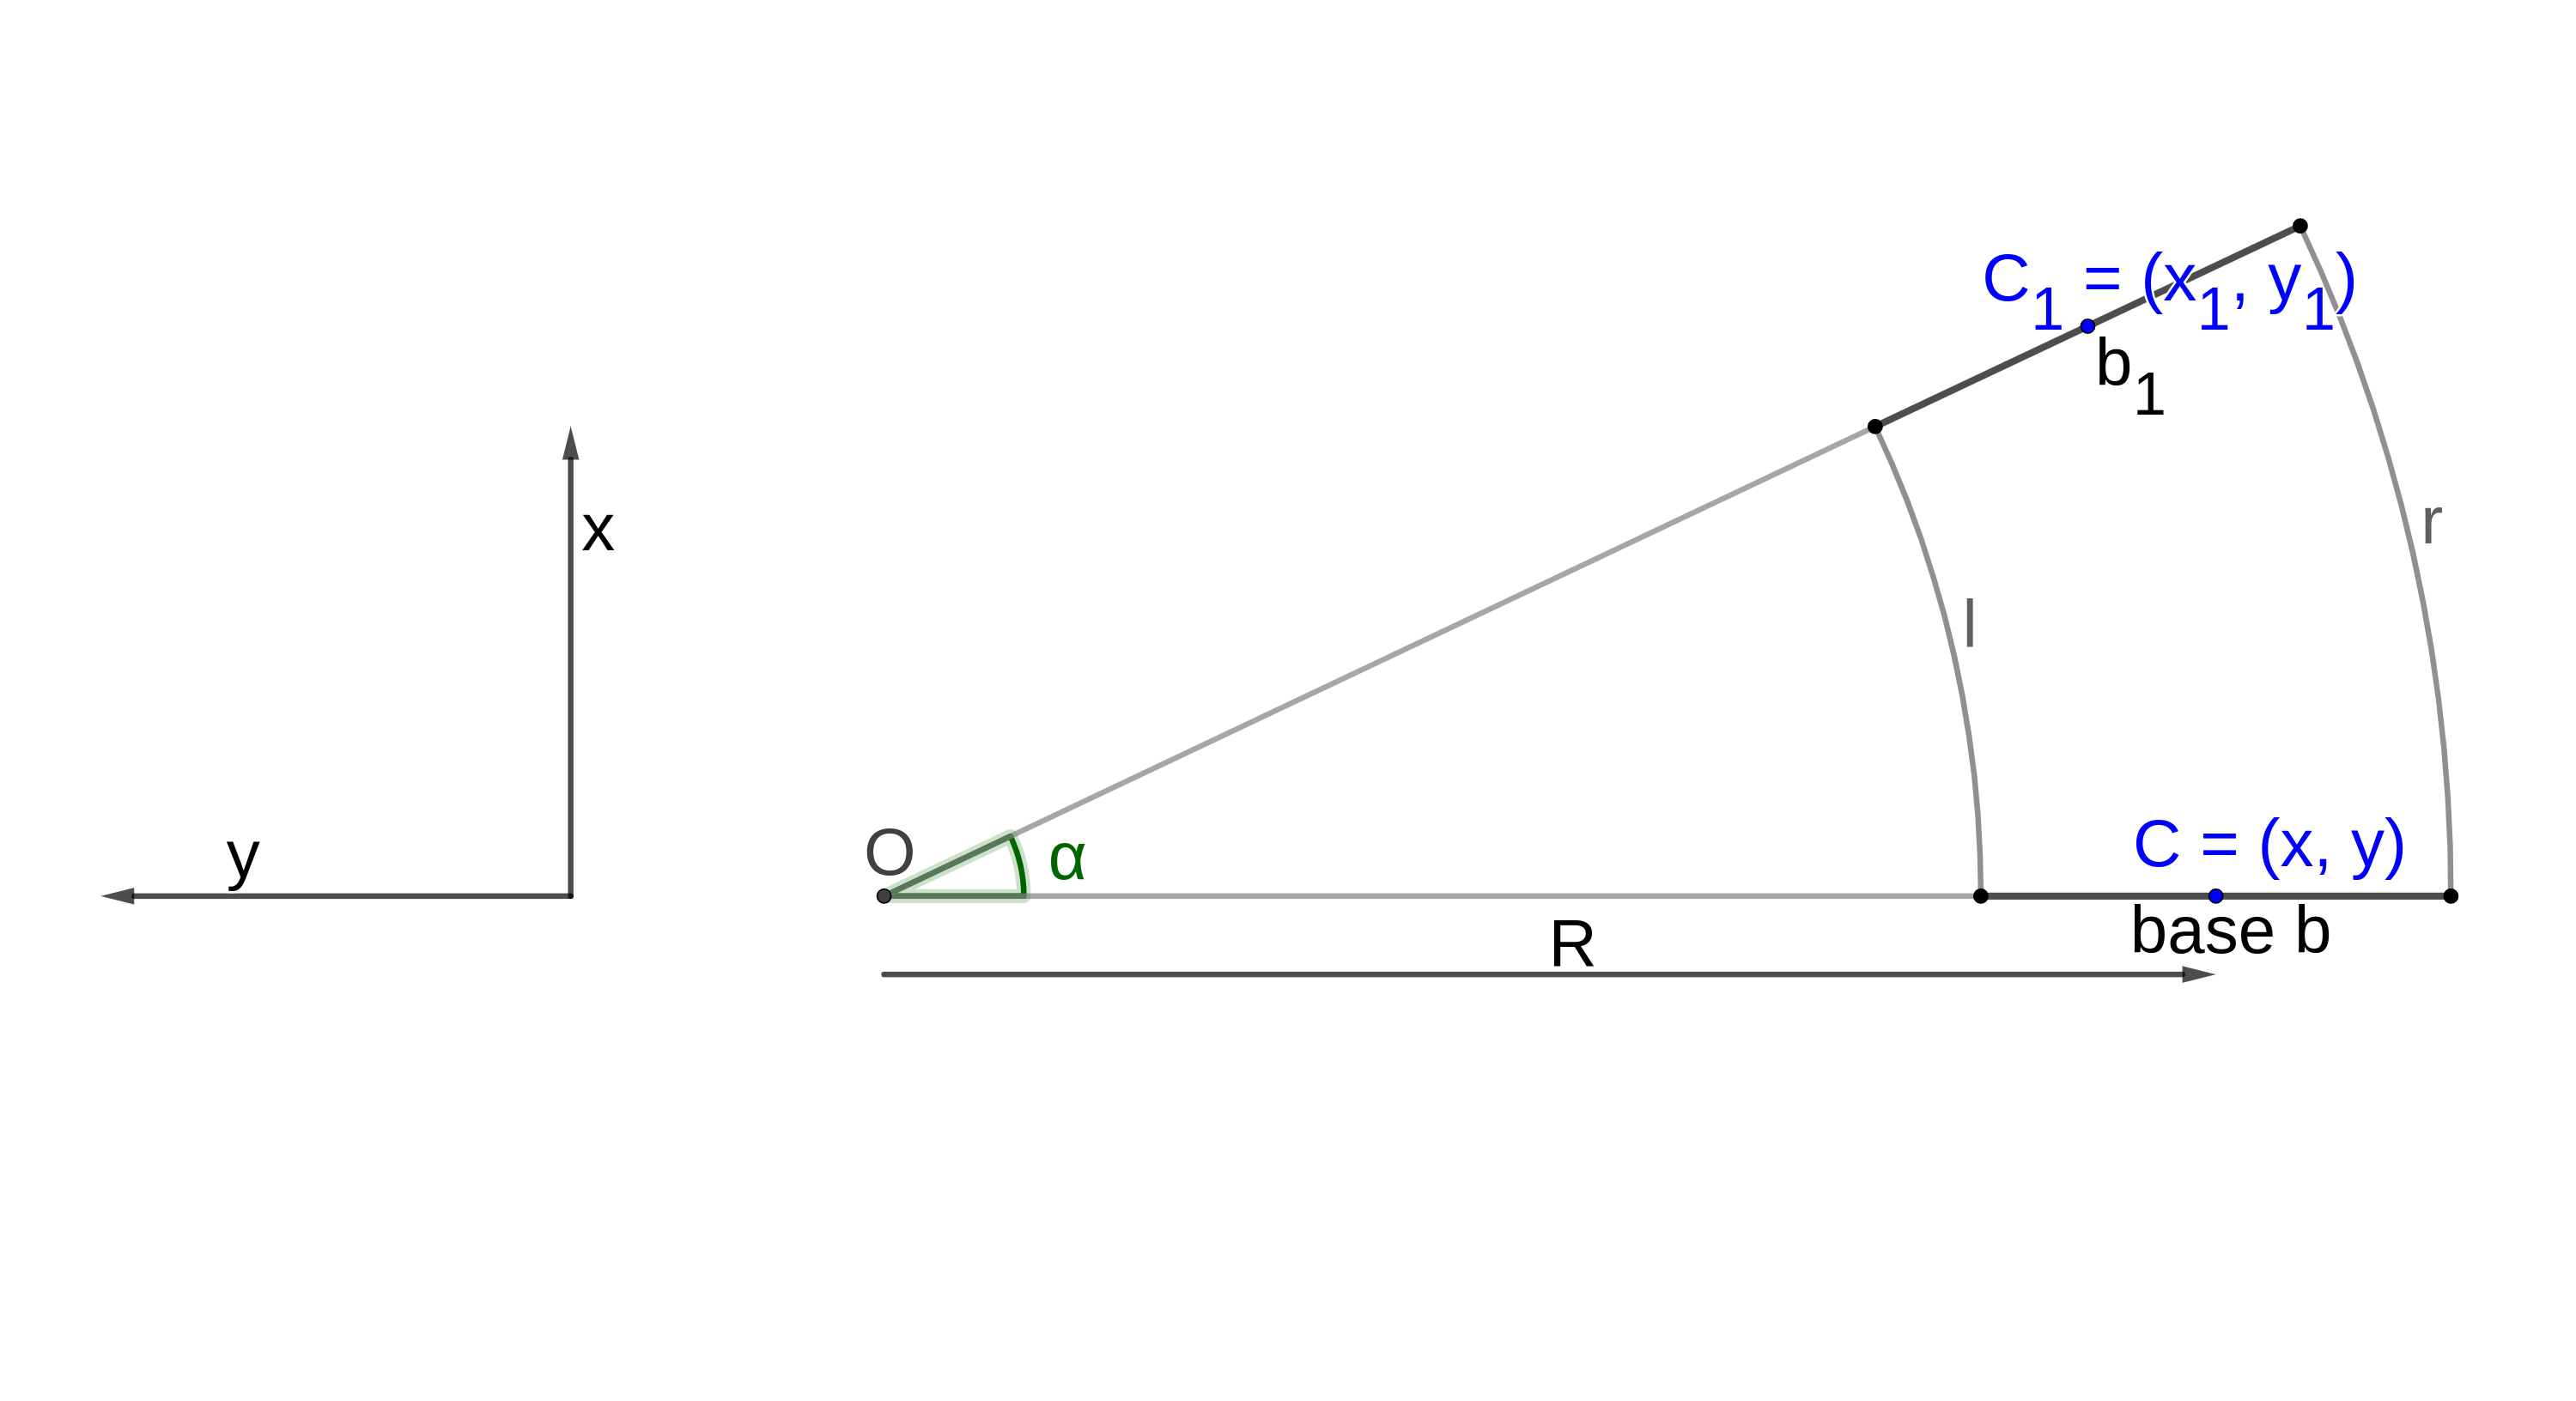
\includegraphics[scale=0.9]{differential_drive_1}
	\captionsetup{justification=centering, margin=1.5cm}
	\centering
	\caption{Model of an instantaneous movement through a rotation.}
	\centering
\end{figure}

Using this model, we can express the local movement of each wheel \textit{l, r} as a function of the parameters of the instant rotation \textit{R, }$\alpha$\footnote{The length of an arc of a circle with radius \textit{r} and subtending an angle $\alpha$ (measured in radians) with the circle center is : \textit{l} = $\alpha$ \textit{r}}.
\begin{gather*}
	r = ( R + \frac{b}{2} ) \alpha\\
	l = ( R - \frac{b}{2} ) \alpha
\end{gather*}
Respectively adding and subtracting these two equations we get:
\begin{gather*}
	r + l = 2 R \alpha\\
	r - l = b \alpha
\end{gather*}
And therefore we are able to express \textit{R, }$\alpha$ as a function of \textit{l, r}:
\begin{align}
	\alpha = \frac{r - l}{b}\\[3mm]
	R = \frac{r + l}{2 \alpha} \label{R}
\end{align}

We are now ready to express the local movement in the local reference frame:
\begin{figure}[!ht]
	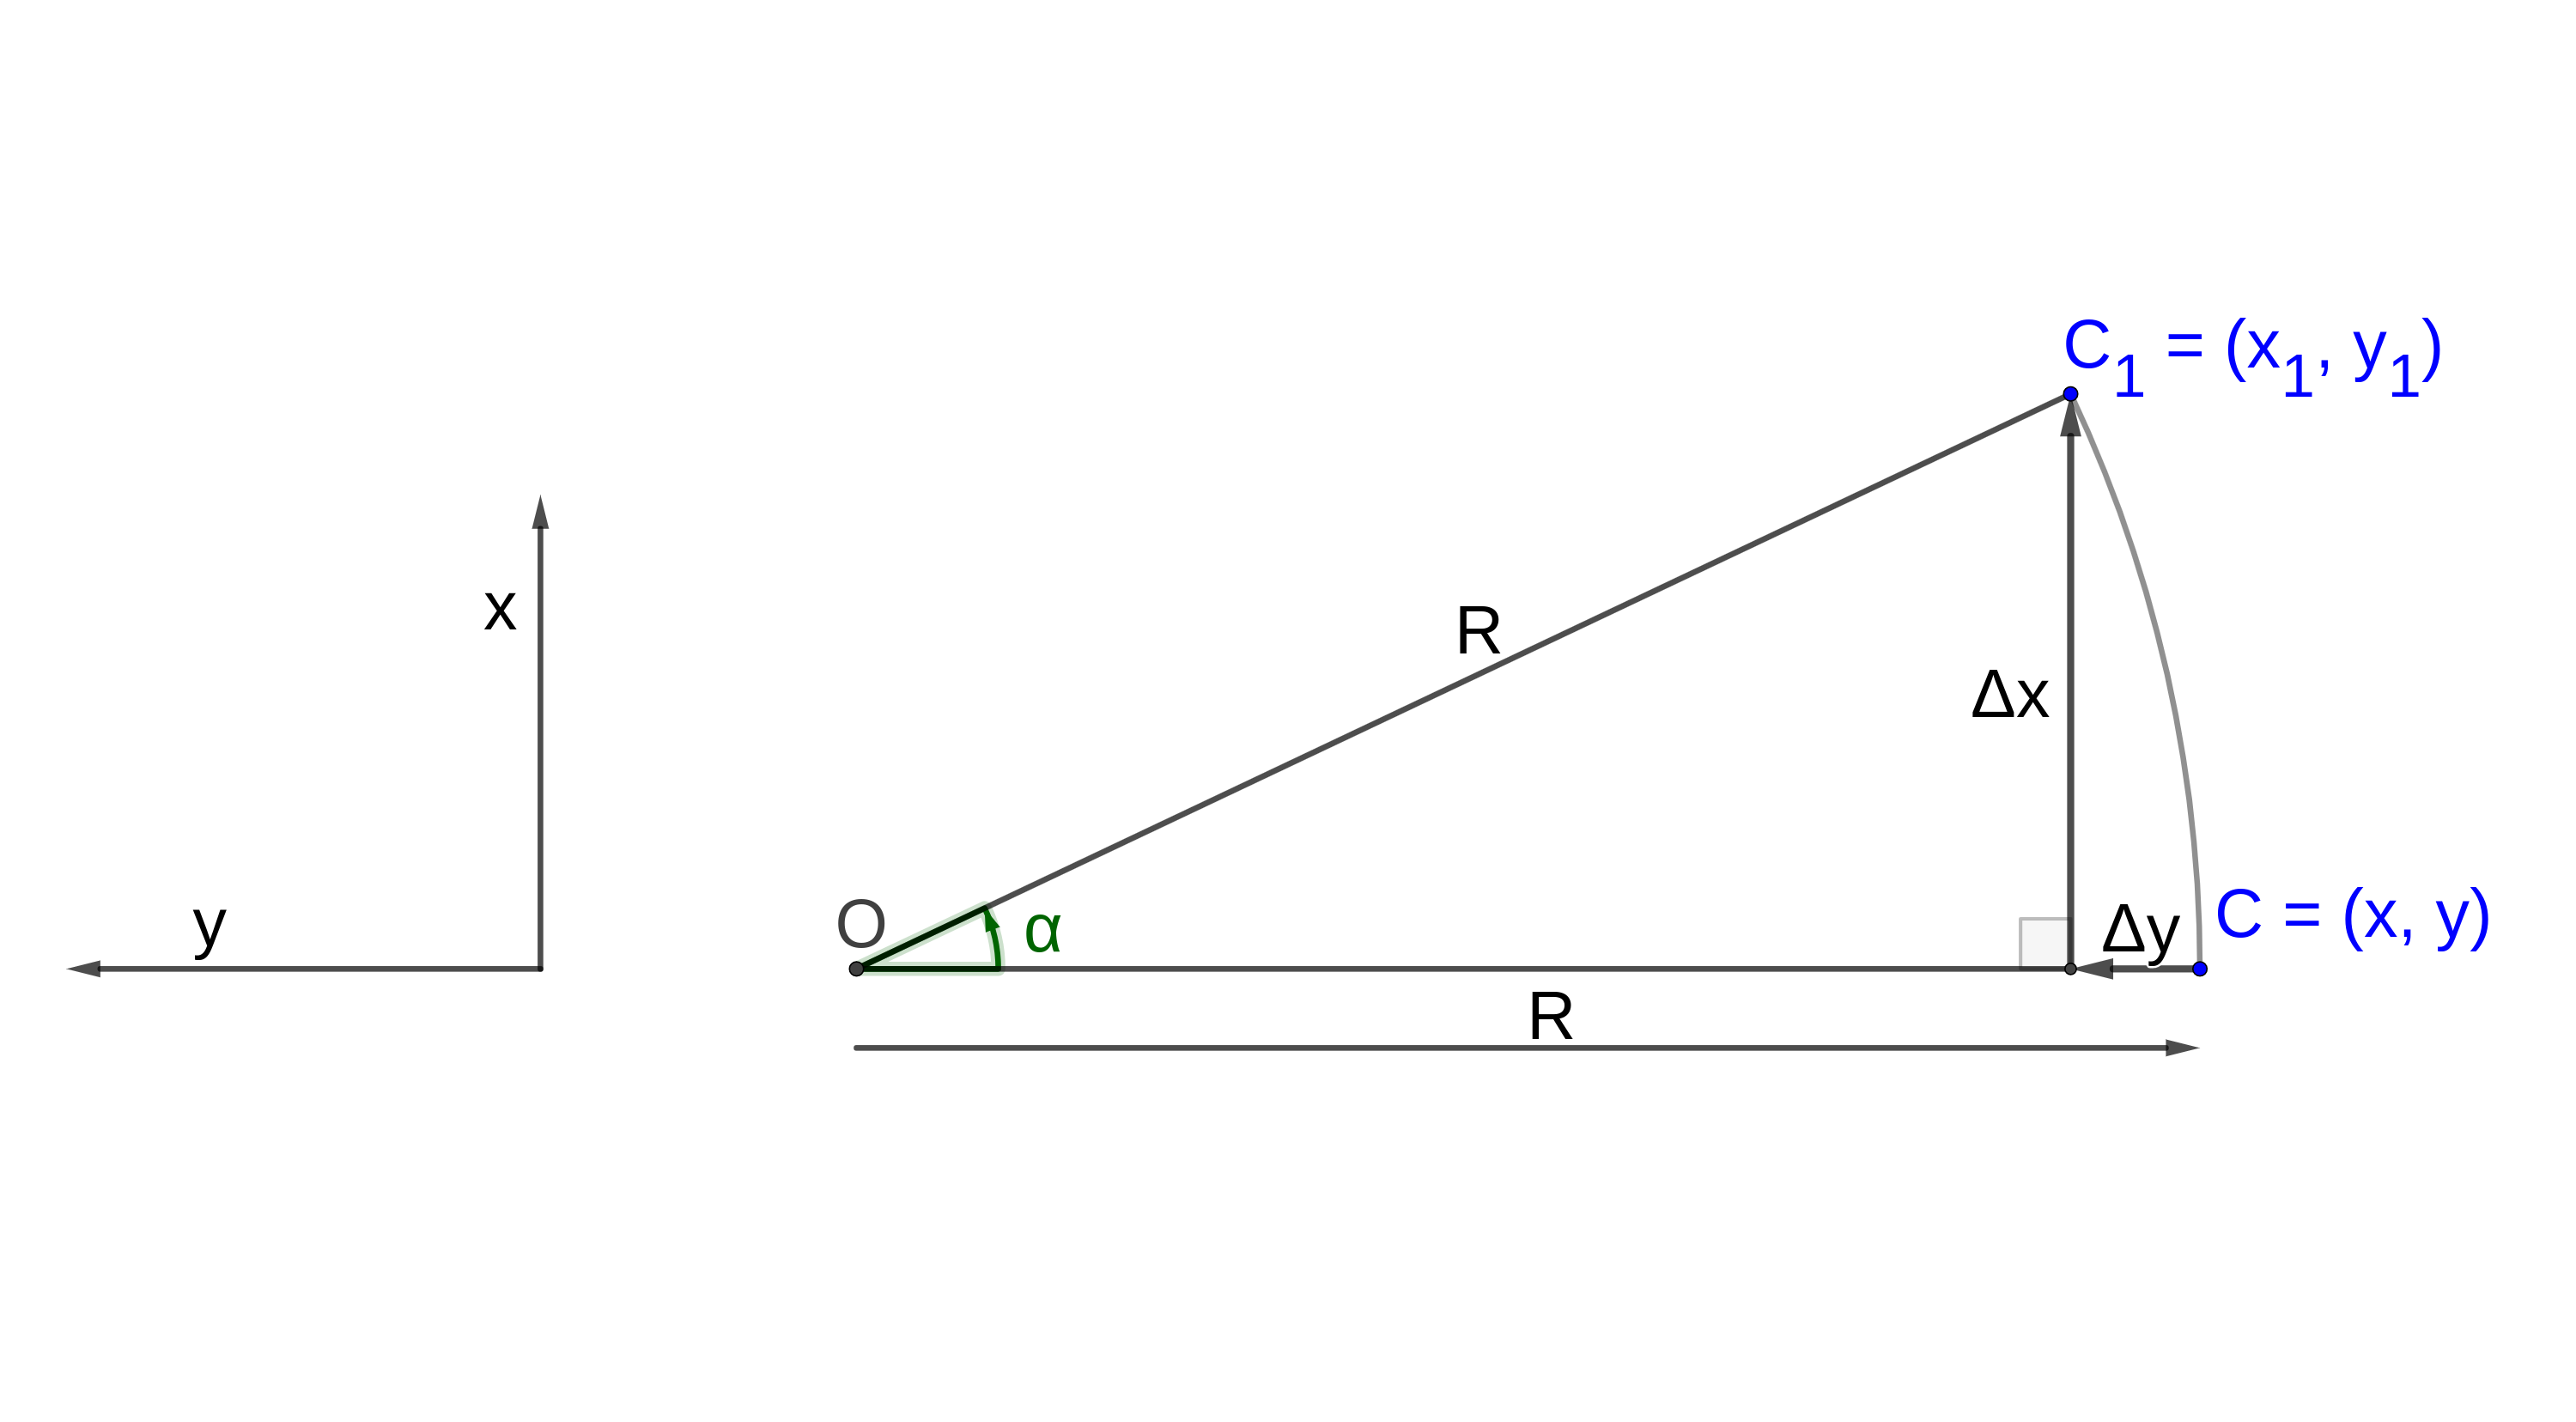
\includegraphics[scale=0.9]{differential_drive_deltas}
	\captionsetup{justification=centering, margin=1.5cm}
	\centering
	\caption{Model of an instantaneous movement through a rotation (emphasis on the local movement).}
	\centering
\end{figure}
\begin{align}
	\Delta x &= R sin \alpha\\
	\Delta y &= R - R cos \alpha = R ( 1 - cos \alpha )
\end{align}

and finally, using the \eqref{R}:

\begin{align}
	\Delta x &= \frac{r + l}{2}\text{ } \frac{sin \alpha}{\alpha}\\[3mm]
	\Delta y &= \frac{r + l}{2}\text{ } \frac{1 - cos \alpha}{\alpha}\\[3mm]
	\Delta \theta &= \alpha
\end{align}

Since $\frac{sin \alpha}{\alpha}$ and $\frac{1 - cos \alpha}{\alpha}$ have a singularity for $\alpha = 0$, we will use the corresponding Taylor-Maclaurin series\footnote{Taylor-Maclaurin series for sine and cosine:\\[1mm] $sin \alpha = \alpha - \frac{1}{3!}\alpha^3 + \frac{1}{5!}\alpha^5 - \frac{1}{7!}\alpha^7 + ...$\\[2mm] $cos \alpha = 1 - \frac{1}{2}\alpha^2 + \frac{1}{4!}\alpha^4 - \frac{1}{6!}\alpha^6 + ...$}:
\begin{align}
	\frac{sin \alpha}{\alpha} &= 1 - \frac{1}{3!}\alpha^2 + \frac{1}{5!}\alpha^4 - \frac{1}{7!}\alpha^6 + ...\\[3mm]
	\frac{1 - cos \alpha}{\alpha} &= \frac{1}{2}\alpha - \frac{1}{4!}\alpha^3 + \frac{1}{6!}\alpha^5 + ...
\end{align}


\subsection{Movement in the Global Reference Frame}\label{from_local_to_global_mov}

Having calculated the local movement, we are ready to integrate the latest sensors' measurements in the robot's global odometry.
\begin{figure}[!ht]
	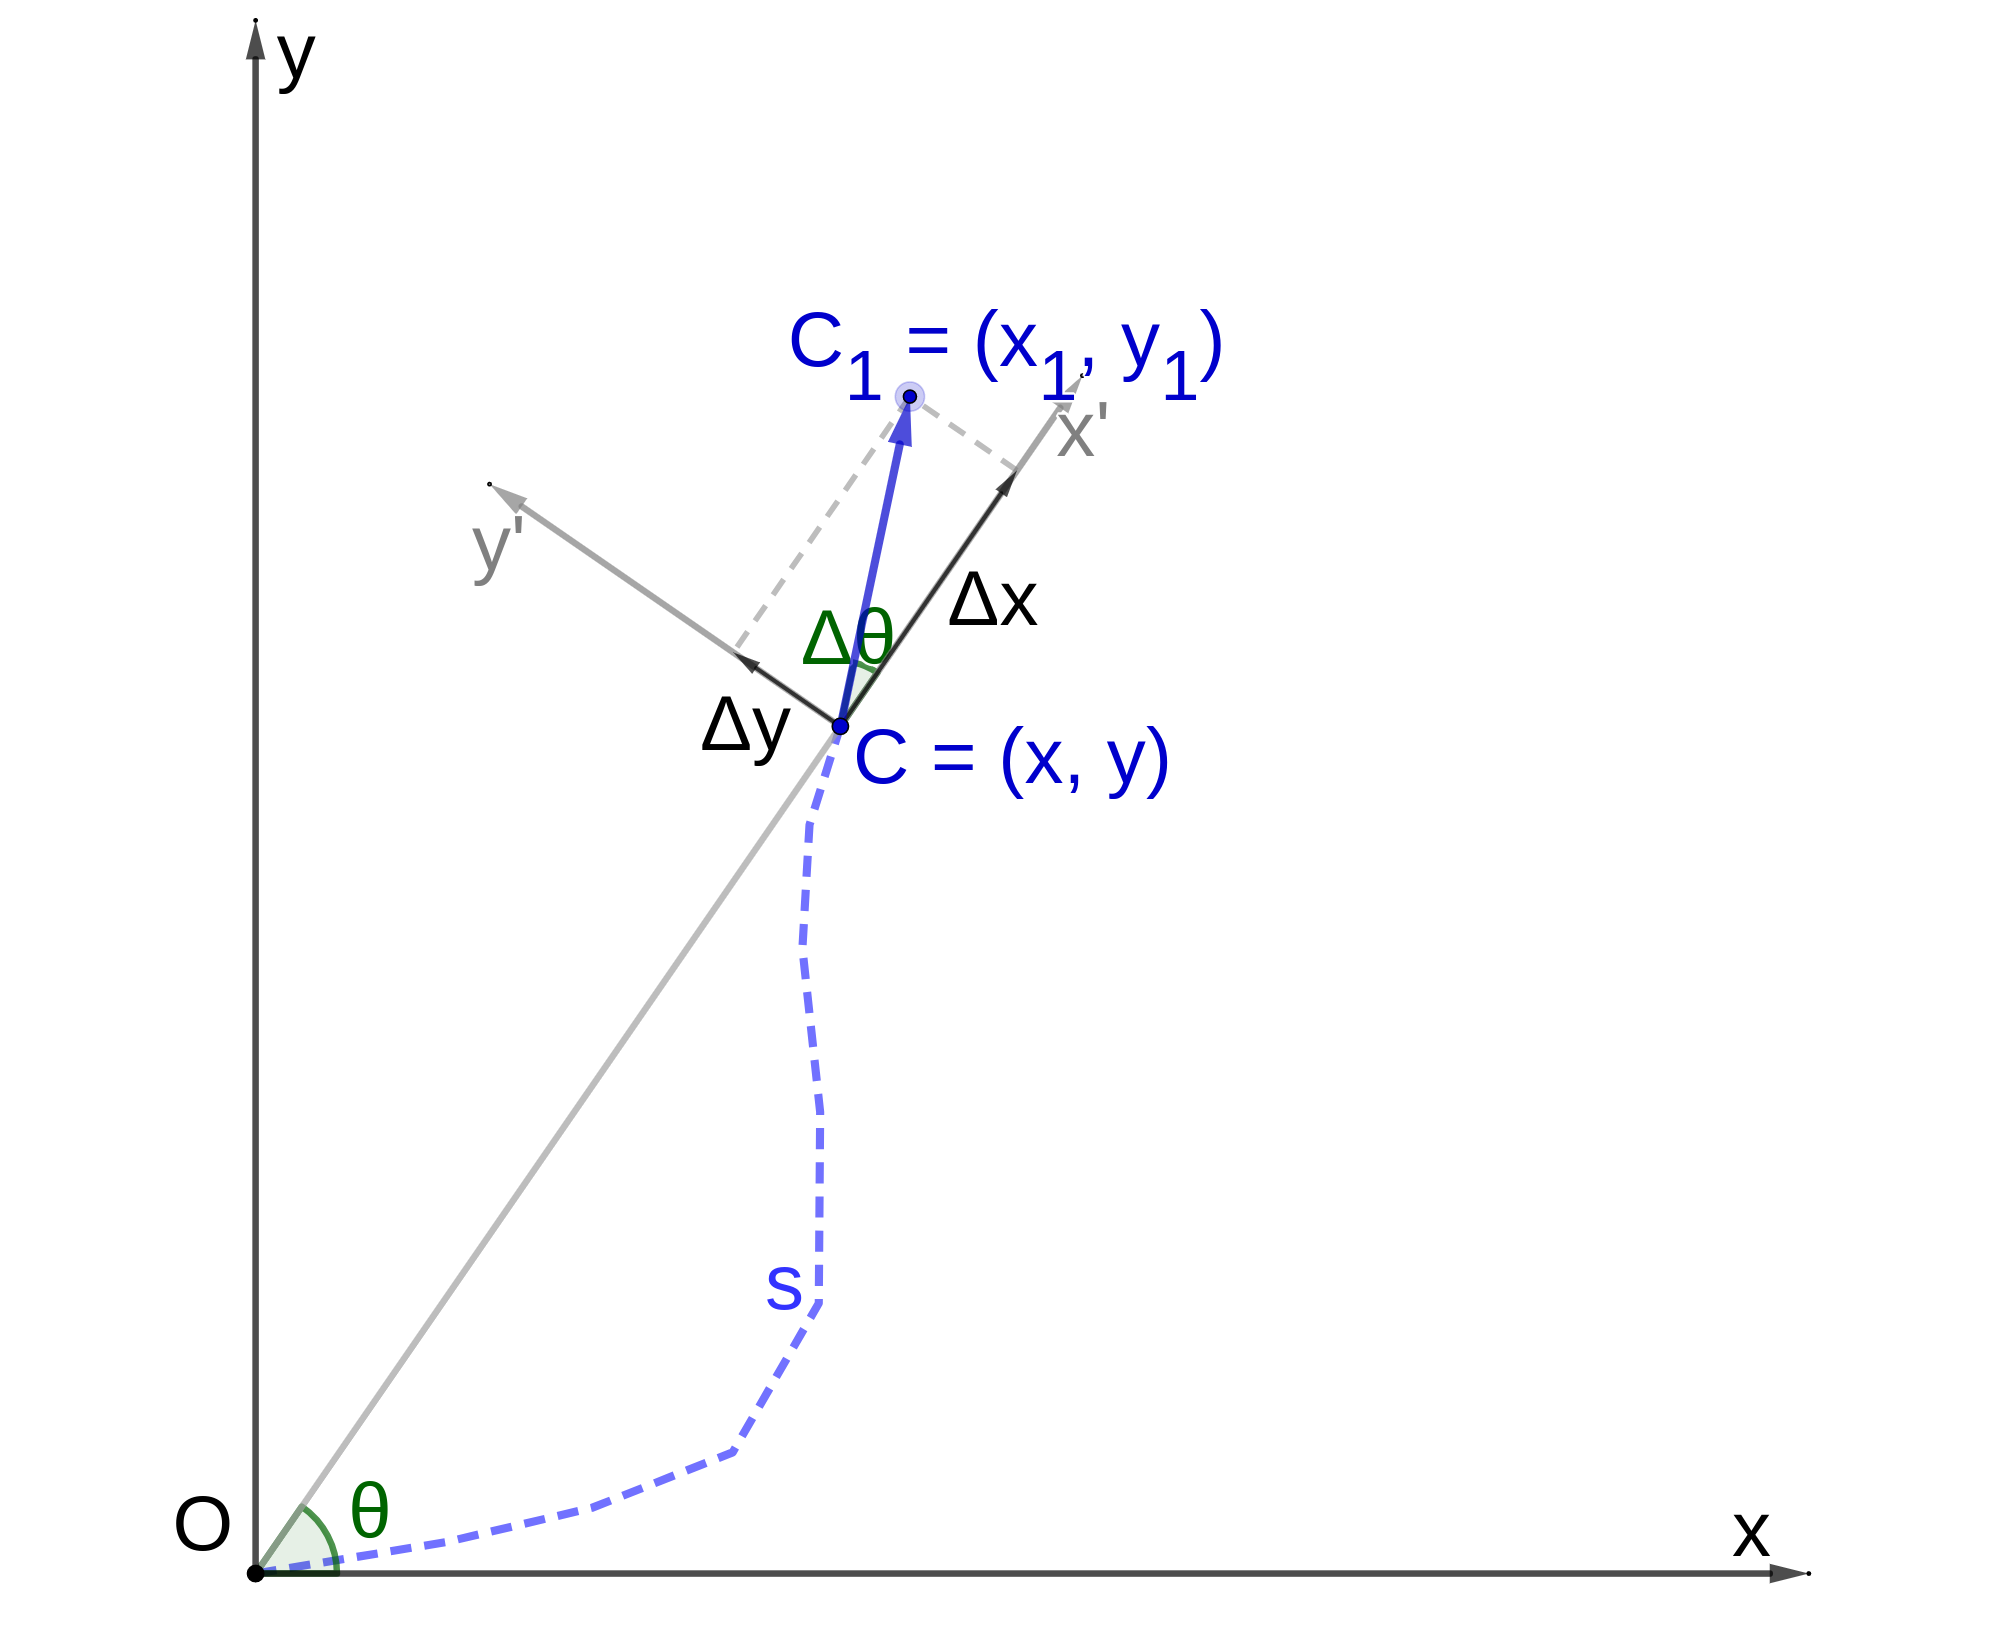
\includegraphics[scale=0.7]{differential_drive_global}
	\captionsetup{justification=centering, margin=1.5cm}
	\centering
	\caption{Movement in the Global Reference Frame.}
	\centering
\end{figure}

\begin{align}
	x &+= \Delta x cos \theta - \Delta y sin \theta\\
	y &+= \Delta x sin \theta + \Delta y cos \theta\\
	\theta &+= \Delta \theta
\end{align}

\subsection{Velocities Update}

To calculate the velocities, we will consider the movement of its central point \textit{C} as the movement fo the robot (using the \eqref{R}).
\begin{align}
	\Delta s = R \alpha = \frac{r + l}{2 \alpha} \alpha = \frac{r + l}{2}
\end{align}
At this point we can also calculate the instant robot's velocities, we will call $v_t$ the translational velocity and $v_r$ the rotational velocity:
\begin{align}
	v_t &= \frac{\Delta s}{\Delta t} = \frac{r + l}{2 \Delta t}\\[3mm]
	v_r &= \frac{\Delta \theta}{\Delta t}
\end{align}

For an implementation of Differential Drive see Appendix \ref{diff_drive_implementation}.

\section{Inertial Navigation}

Inertial navigation is a navigation technique in which the measurements provided by the accelerometer and the gyroscope are used to update the estimate of the current position and orientation of the robot with respect to a known starting point.\supercite{intro_inertial_navigation}

\subsection{Dead Reckoning}

As mentioned in Section \ref{imu_integration}, to keep track of the orientation of the robot we need to integrate the gyroscope measurements, while to keep track of the position we can integrate the accelerometer measurements obtaining the local displacement and then project it on the global axes (using the orientation determined using the gyroscope measurements).

\subsubsection{Updating Orientation}

At each sampling time interval, the gyroscope gives us the observation of the angular velocity of the robot.\\
Therefore since we observe $v_r = \der{\theta}{t}$, the integration is immediate:
\begin{align}
	\theta += v_r \Delta t
\end{align}

\subsubsection{Updating Position}

At each sampling time interval, the accelerometer provides observations on the translational accelerations along the x-axis and the y-axis of the local reference frame.\\

We will first of all calculate the instant movement in the local reference frame:
\begin{align}
	\Delta x &= v_x \Delta t + \frac{1}{2} a_x \Delta t ^ 2\\
	\Delta y &= v_y \Delta t + \frac{1}{2} a_y \Delta t ^ 2
\end{align}

At this point we can project it onto the global axes, calculating the displacement in the global reference frame (in a similar way as we did for the differential drive in Section \ref{from_local_to_global_mov}):
\begin{align}
	x &+= \Delta x cos \theta - \Delta y sin \theta\\
	y &+= \Delta x sin \theta + \Delta y cos \theta
\end{align}

\subsection{High-pass filter}

However this basic navigation algorithm is very inaccurate. One of the main reasons is that the IMU is subject to electromagnetic noise and therefore will measure non-zero accelerations and rotations even if the robot is not moving.\\
This problem is far more evident for the position rather than for the orientation, due to the double integration in the navigation algorithm which increases the error.\\

The first solution we have adopted is a simple high-pass filter, hence we ignore translational accelerations and rotational velocities below a predefined threshold ($\sim$0.4 DPS\footnote{DPS stands for Degrees Per Second} for rotational velocities and $\sim$0.05 G-Forces for translational accelerations).
\begin{figure}[!ht]
	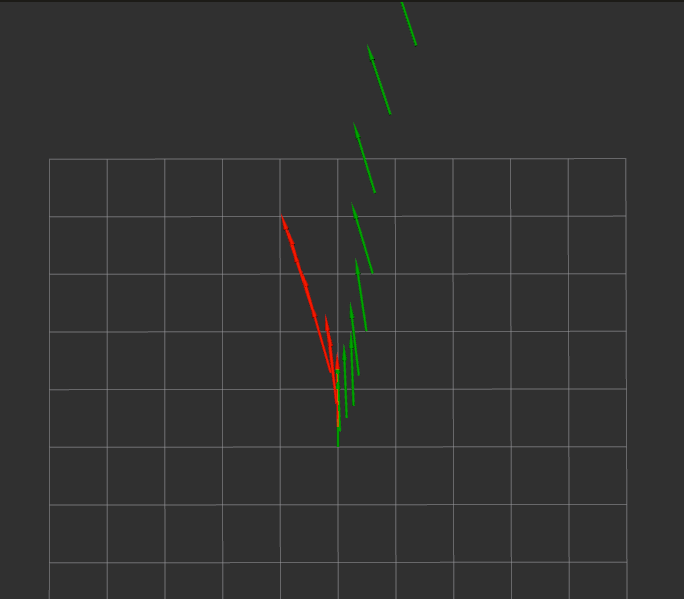
\includegraphics[scale=0.4]{encs_imu_000_trans_vel_x_y}
	\captionsetup{justification=centering, margin=1.5cm}
	\centering
	\caption{Inertial Navigation (with high-pass filter) trajectory (in green) compared to the more accurate Differential Drive trajectory (in red) visualized using Rviz.}
	\centering
\end{figure}


\subsection{Stop Motion detection}

Using the described high pass filter we have obtained a more accurate result, however once this localization algorithm has detected the movement of the robot, it is not able to detect when the robot stops. This is because even if the accelerometer no longer detects any acceleration, the previous accelerations have produced a non-zero velocity that will hardly be zeroed when the robot stops.\\

\begin{figure}[!ht]
	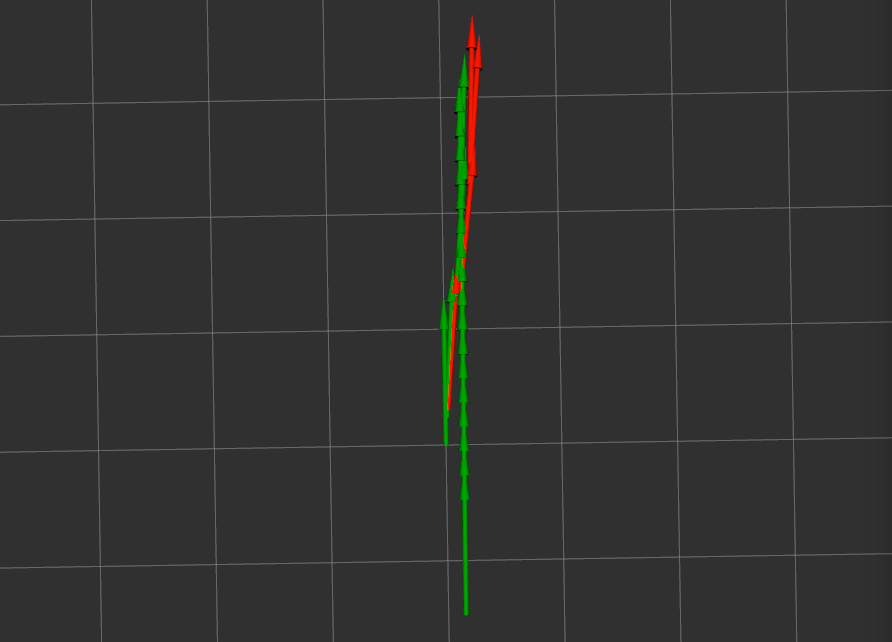
\includegraphics[scale=0.4]{encs_imu_004_imu_decel_to_neg_vel}
	\captionsetup{justification=centering, margin=1.5cm}
	\centering
	\caption{Inertial Navigation trajectory (in green) compared to the more accurate Differential Drive trajectory (in red) visualized using Rviz. We can notice how after a first phase in which the Inertial Navigation odometry followed the Differential Drive odometry, the former was unable to detect the motionless state and (having a negative velocity due to the braking phase) brought the odometry back beyond the starting position before we stopped the visualization.}
	\centering
\end{figure}

Therefore we designed a \textit{Stop Motion Detection Algorithm} which basically counts the instants with positive and negative acceleration between two motionless states and the consecutive instants with zero acceleration for each axis.\\
When the number of consecutive instants with no acceleration exceeds the difference between the instants with positive and negative acceleration scaled by a predefined factor, we assume that the robot is motionless due to friction and therefore we zero its velocity.\\
\begin{ccode}
	#define STOP_ZERO_ACCEL_OUTLIER_FILTER 5
	#define STOP_BREAKING_TRESHOLD 2

	if ( translational_acceleration_x_axis > 0. ) {
		total_time_pos_accel_x++;
		curr_time_zero_accel_x = 0;
	} else if ( translational_acceleration_x_axis < 0. ) {
		total_time_neg_accel_x++;
		curr_time_zero_accel_x = 0;
	} else //accel_x_axis == 0.
		curr_time_zero_accel_x++;	
	
	if( curr_time_zero_accel_x > STOP_ZERO_ACCEL_OUTLIER_FILTER &&
			curr_time_zero_accel_x >= abs( total_time_pos_accel_x - total_time_neg_accel_x) * STOP_BREAKING_TRESHOLD) {
		//after it has had approximately
			//the same time of positive and negative acceleration
			//we assume it is in STATIONARY state
		translational_acceleration_x_axis = 0.;
		translational_velocity_x_axis = 0.;
		
		//we reset the variables
		total_time_pos_accel_x = 0;
		total_time_neg_accel_x = 0;
	}
\end{ccode}
\captionof{lstlisting}{Implementation of the described Stop Motion Detection algorithm.}


\begin{figure}[htb]
 \centering
	\begin{subfigure}{0.3\textwidth}
		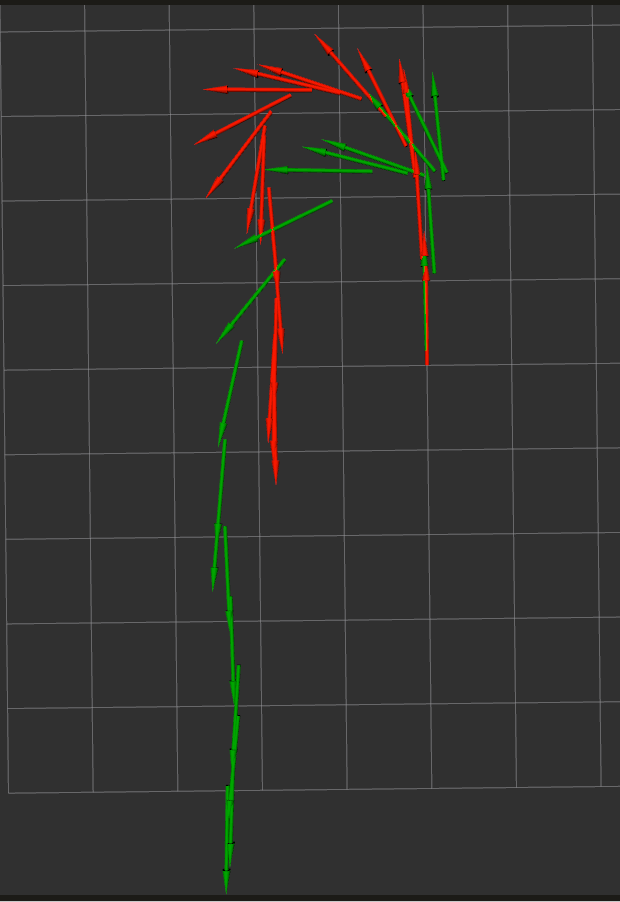
\includegraphics[width=\linewidth]{imu_encs_006_stop_motion_detecion_x_y_full}
	\end{subfigure}\hfil
	\begin{subfigure}{0.3\textwidth}
		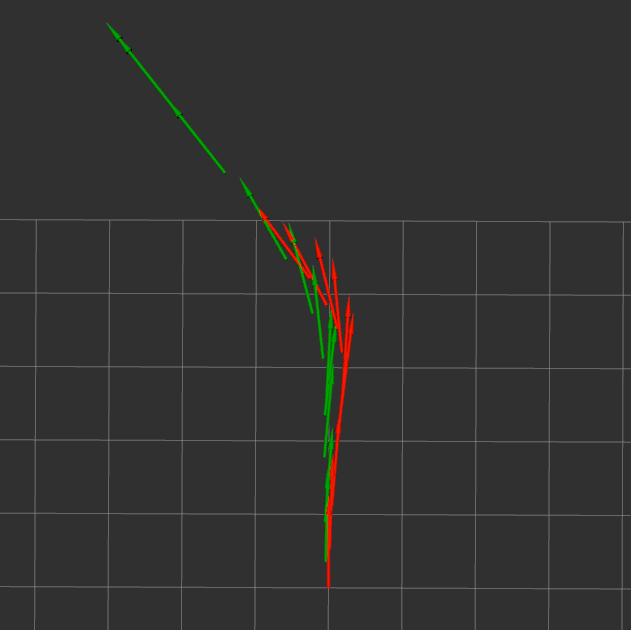
\includegraphics[width=\linewidth]{imu_encs_006_stop_motion_detection}
	\end{subfigure}\hfil
	\begin{subfigure}{0.3\textwidth}
		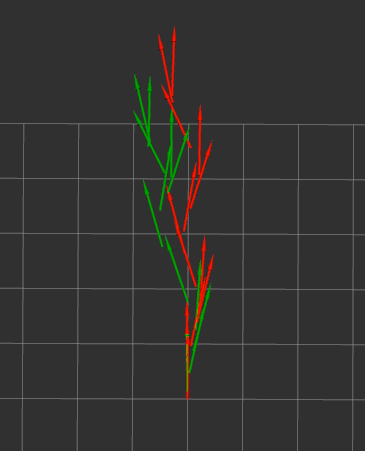
\includegraphics[width=\linewidth]{imu_encs_010_stop_motion}
	\end{subfigure}
	\captionsetup{justification=centering, margin=1.5cm}
	\caption{Inertial Navigation (with Stop Motion Detection) trajectories (in green) compared to the more accurate Differential Drive trajectories (in red) visualized using RViz.}
	\label{stop_motion_fig}
\end{figure}
In the images \ref{stop_motion_fig}, we can see how the Inertial Navigation technique, even with the high-pass filter and the Stop Motion Detection, is far less accurate than the Differential Drive technique; however it is now able to detect a motionless state, eventually with some latency, without moving the odometry to infinity.

For an implementation of Inertial Navigation see Appendix \ref{inert_nav_implementation}.
